% Created 2022-10-27 Thu 16:38
% Intended LaTeX compiler: xelatex
\documentclass[9pt,aspectratio=169]{beamer}
\usepackage{graphicx}
\usepackage{longtable}
\usepackage{wrapfig}
\usepackage{rotating}
\usepackage[normalem]{ulem}
\usepackage{amsmath}
\usepackage{amssymb}
\usepackage{capt-of}
\usepackage{hyperref}
\usepackage{fontspec}
\setsansfont{Archivo Expanded}
\setmainfont{Lora}
\setmonofont{PragmataPro Liga}
\definecolor{UOBred}{rgb}{0.6706, 0.1216, 0.1765}
\setbeamercolor{palette primary}{bg=UOBred, fg=white}
\setbeamercolor{palette secondary}{bg=UOBred, fg=white}
\setbeamercolor{palette tertiary}{bg=UOBred, fg=white}
\setbeamercolor{palette quaternary}{bg=UOBred, fg=white}
\setbeamercolor{structure}{fg=UOBred}
\setbeamercolor{structure}{fg=UOBred}
\usetheme{default}
\usefonttheme[stillsansseriflarge]{serif}
\author{Joseph Hallett}
\date{\today}
\title{Why software engineers don't get bonuses}
\titlegraphic{
\includegraphics[height=0.5cm]{bristol.png}}
\hypersetup{
 pdfauthor={Joseph Hallett},
 pdftitle={Why software engineers don't get bonuses},
 pdfkeywords={},
 pdfsubject={},
 pdfcreator={Emacs 28.2 (Org mode 9.5.5)}, 
 pdflang={English}}
\begin{document}

\maketitle

\begin{frame}[label={sec:org03989aa}]{Abstraction, abstraction\ldots{}}
In computer science we like to pretend that it's all digital\ldots{}
\begin{itemize}
\item Perfect 1s and 0s.
\item Computers that work exactly how the specifications say.
\item Hardware can be (largely) ignored.
\item Lower level details\ldots{} \emph{that's for electrical engineers not us!}
\end{itemize}

\begin{block}{This doesn't always work out.}
\end{block}
\end{frame}

\begin{frame}[label={sec:orgb0a1e9e},fragile]{Money, money, money\ldots{}}
 It mostly works out though\ldots{}
\begin{itemize}
\item But this whole unit is about what happens when computers start doing weird things.
\end{itemize}

\begin{block}{Electrical engineers, and computer architects make mistakes}
Cost of fixing hardware is big
\begin{itemize}
\item You cannot trivially fix a silicon wafer
\item You cannot recall old hardware and change the circuits
\end{itemize}

Cost of fixing software is cheap
\begin{itemize}
\item It's just code!
\end{itemize}
\end{block}

\begin{block}{When there is a bug\ldots{} its the software engineers who fix it}
Consequently we have to clean up after their messes
\begin{itemize}
\item So software is always running late
\item So we don't get a bonus \texttt{:-(}

\vfill
\footnotesize
\end{itemize}
(or so said my first boss)
\end{block}
\end{frame}

\begin{frame}[label={sec:orgfdfc2ab}]{Plan}
In this lecture we'll cover two ways hardware is broken.
\begin{itemize}
\item Rowhammer and DRAM
\item Meltdown/Spectre and CPUs
\end{itemize}

We'll also cover how software works around it.
\end{frame}

\begin{frame}[label={sec:org7f9c78b}]{DRAM glorious, DRAM!}
Memory! Used to store all the things the computer is thinking about
that we can't fit in a register!
\begin{itemize}
\item Implemented using a \emph{capacitor} and a \emph{transistor} per bit
\item \emph{Ganged} (arranged) into long rows (\textasciitilde{}8k bits per row)
\item Placed into \emph{banks} of ganged rows
\end{itemize}

When we want to read a bit of memory:
\begin{itemize}
\item We find the row it is in.
\item Activate the row by letting the capacitors discharge
\item Which copies the row into an active memory buffer
\end{itemize}

DRAM needs to be \emph{refreshed} so the capactiors don't lose their charge over time
\begin{itemize}
\item Roughly every 64ms for modern hardware
\end{itemize}
\end{frame}

\begin{frame}[label={sec:org9f302cd}]{Electronic Engineering is messy}
\begin{block}{Capacitors leak charge}
\end{block}

\begin{block}{Current in wires induces current in other nearby wires}
\end{block}

\begin{block}{The 1s and 0s aren't charged or uncharged capacitors}
\begin{itemize}
\item Its whether a capacitor is currently discharging more or less than a
threshhold voltage
\end{itemize}

But this is all fine because electronic components are large!
\end{block}
\end{frame}

\begin{frame}[label={sec:org14f8436}]{Or they were\ldots{}}
\begin{itemize}
\item As memory capacity has \emph{increased}\ldots{}
\item The physical dimensions of memory has got \emph{smaller}.

\vfill
\begin{quote}
``The \sout{Dwarves} \alert{Electrical engineers} tell no tale; but even as \sout{mithril}
\alert{memory density} was the foundation of their wealth, so also it was
their destruction: they delved too greedily and too deep, and
disturbed that from which they fled, \sout{Durin's Bane} \alert{Rowhammer}."

--- \alert{Gandalf the Greyhat}
\end{quote}
\end{itemize}
\end{frame}

\begin{frame}[label={sec:org6fc911e}]{Flipping bits}
\begin{columns}
\begin{column}[t]{0.49\columnwidth}
\begin{center}
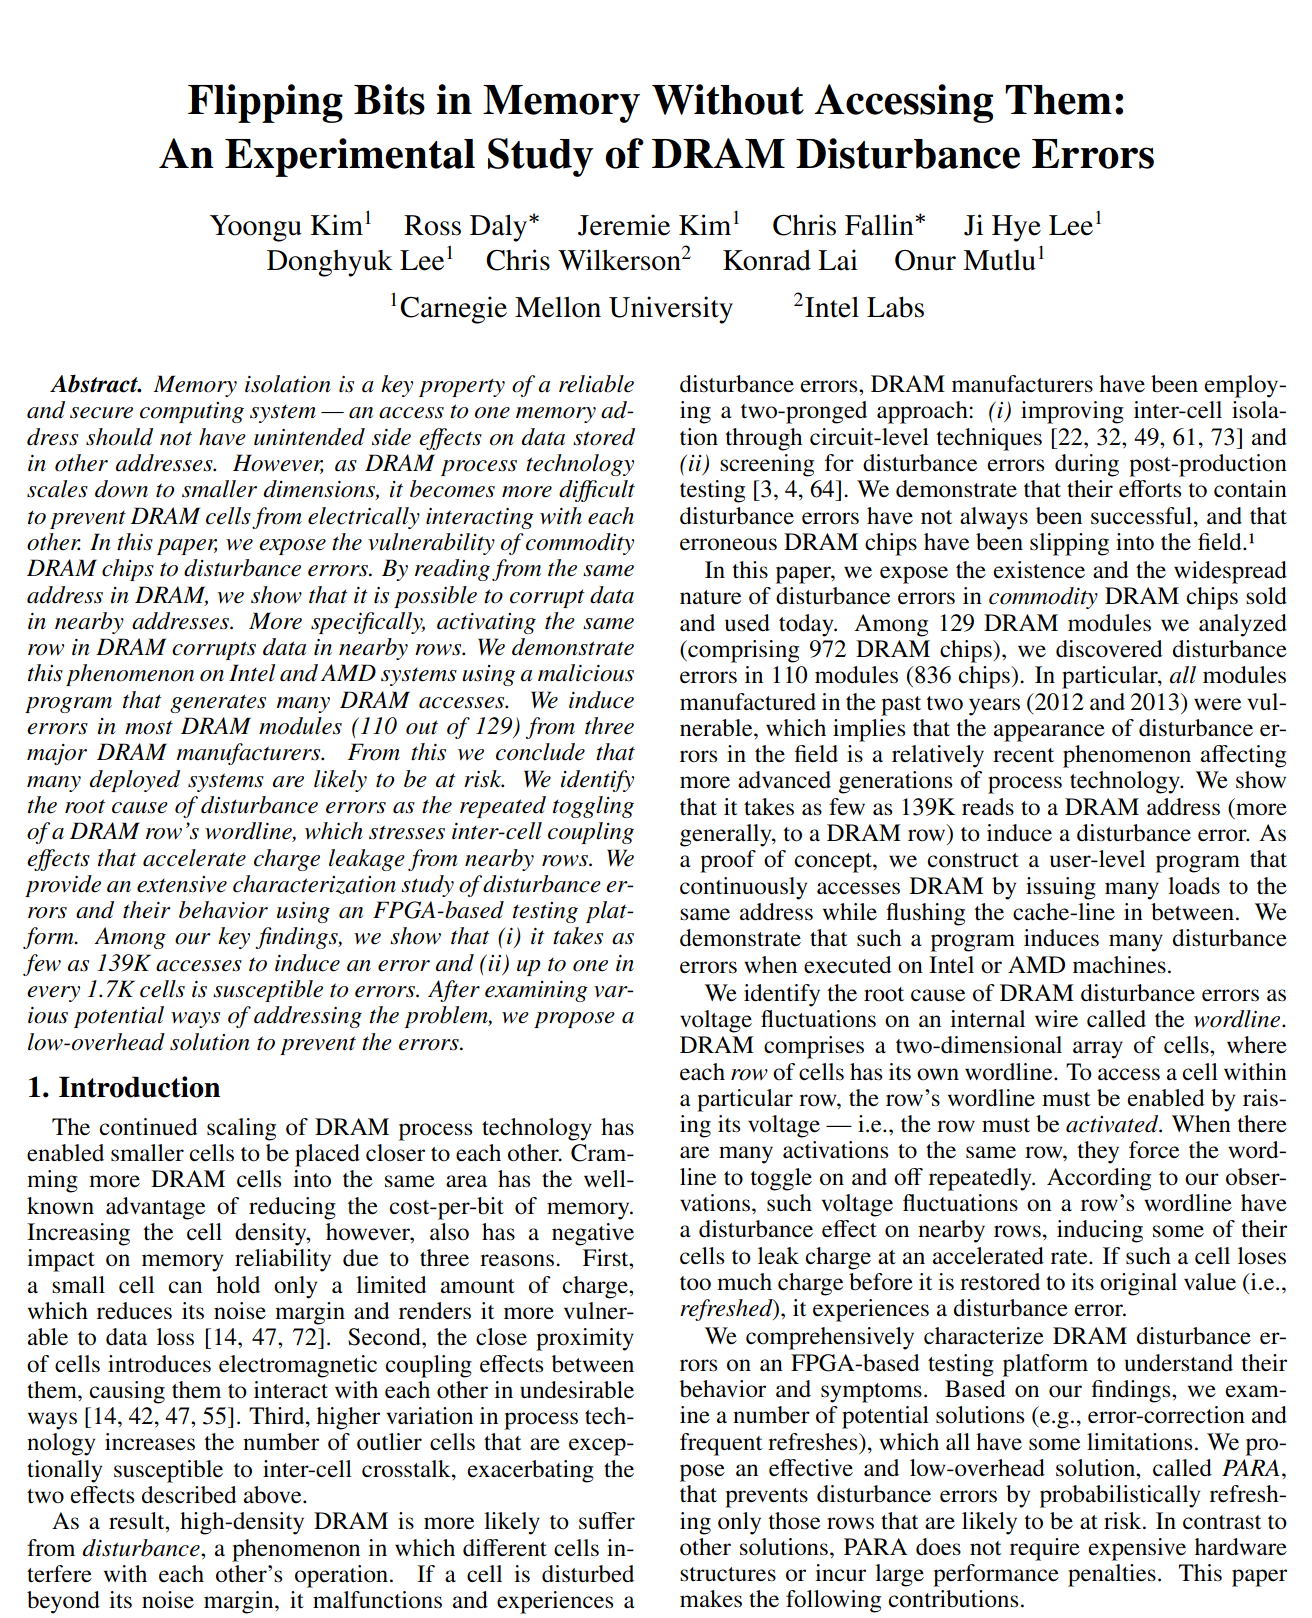
\includegraphics[width=.9\linewidth]{./flippingbits.png}
\end{center}
\end{column}

\begin{column}[t]{0.49\columnwidth}
Rowhammering is a well known bug in DRAM chips since \textasciitilde{}2010

\begin{block}{If you repeatedly charge and discharge a row in DRAM really quickly it can cause errors in nearby rows}
Manufacturers all knew about it, but didn't really bother to document it.
\begin{itemize}
\item Seen as a \emph{reliability} issue, not a \emph{security} issue
\item Cached memory largely fixes it.
\end{itemize}

Several papers discuss it and explore it
\begin{itemize}
\item Almost all RAM is vulnerable to it (to some extent)
\item \emph{Maybe} you could do something malicious theoretically?
\item Still treated as a \emph{reliability} issue
\end{itemize}
\end{block}
\end{column}
\end{columns}
\end{frame}

\begin{frame}[label={sec:org94af626},fragile]{Flipping bits, in practice}
 \begin{columns}
\begin{column}[t]{0.49\columnwidth}
\begin{verbatim}
code1a:
        mov eax, [X]
        mov ebx, [Y]
        clrflush [X]
        clrflush [Y]
        mfence
        jmp code1a
\end{verbatim}
\end{column}

\begin{column}[t]{0.49\columnwidth}
Find two memory addresses X and Y that are in separate rows of RAM and:
\begin{enumerate}
\item Load \texttt{*X} into the active buffer
\item Load \texttt{*Y} into the active buffer
\item Kick \texttt{*X} out of the cache (so next read goes directly to RAM)
\item Kick \texttt{*Y} out of the cache (so next read goes directly to RAM)
\item Ensure that the cache is really gone
\item Repeat (as fast as you can)
\end{enumerate}
\end{column}
\end{columns}
\end{frame}

\begin{frame}[label={sec:orga0581ee},fragile]{Token ASCII Art Diagram}
 \begin{columns}
\begin{column}[t]{0.2\columnwidth}
\begin{verbatim}
   ⋮    |      ! |
        +--------+
Row n+0 |        <- X
        +--------+
Row n+1 | !      |
        +--------+
Row n+2 |        | 
        +--------+
Row n+3 |      ! | 
        +--------+
Row n+4 |        <- Y
        +--------+
   ⋮    |    !   |

        +--------+
Active  |X/Y/X/Y/|
        +--------+
\end{verbatim}
\end{column}

\begin{column}[t]{0.79\columnwidth}
If you perform the rowhammer with the above RAM layout
\begin{itemize}
\item \emph{Eventually} you'll get errors in the adjacent rows (the \texttt{!}'s)
\item This is called \emph{single-sided} Row Hammering
\end{itemize}
\end{column}
\end{columns}
\end{frame}

\begin{frame}[label={sec:orgd3b1901},fragile]{Double Sided Rowhammering}
 \begin{columns}
\begin{column}[t]{0.2\columnwidth}
\begin{verbatim}
   ⋮    |        |
        +--------+
Row n+0 |      ! |
        +--------+
Row n+1 |        <- X
        +--------+
Row n+2 |!!!!!!!!| 
        +--------+
Row n+3 |        <- Y 
        +--------+
Row n+4 |   !    |   
        +--------+
   ⋮    |        |

        +--------+
Active  |X/Y/X/Y/|
        +--------+
\end{verbatim}
\end{column}

\begin{column}[t]{0.79\columnwidth}
If you select \texttt{X} and \texttt{Y} so there is excactly 1 row between them
\begin{itemize}
\item \emph{Eventually} you'll get errors in the adjacent rows (the \texttt{!}'s)
\item \emph{Quickly} you'll get errors in the in-between row
\item This is called \emph{double-sided} Row Hammering
\end{itemize}
\end{column}
\end{columns}
\end{frame}

\begin{frame}[label={sec:orgb351906}]{So what?}
So we can introduce (typically) single bit errors in RAM\ldots{} so what?

\begin{block}{Mark Seaborne and Halvar Flake (and others) continue exploring}
\begin{itemize}
\item Discover double-sided variant of Rowhammering
\item Find that its not just all RAM which is susceptible to this, but that its \emph{all rows} in \emph{all ram} (between 30--100\%\ldots{} but improvements later make it 100\%).
\end{itemize}

They discover the bit flips are consistent
\begin{itemize}
\item Same bits flip every time when you Rowhammer the same rows
\end{itemize}

And even consistent between the same RAM products
\begin{itemize}
\item If Alice and Bob have the same make RAM from the same manufacturer
\item Then if they Rowhammer the same rows the same bits will always flip
\end{itemize}
\end{block}
\end{frame}

\begin{frame}[label={sec:orgce2ddae}]{This seems bad, but so what?}
\begin{itemize}
\item You can violate the integrity of RAM, but is that all?
\item How could you possibly use this as part of an attack to get arbitrary code execution?
\end{itemize}
\end{frame}

\begin{frame}[label={sec:orgaef14d4},fragile]{NaCl Sandbox}
 \emph{Privileged} sandbox for running \emph{native code} from a web browser safely.
\begin{itemize}
\item Checks if the code is \emph{safe} (i.e. doesn't contain any weird syscalls or violate safety properties)
\item If so, it loads the chunks of instructions aligned on 32B boundaries
\end{itemize}

\begin{verbatim}
and eax, 0x000F                 ; Truncate address to 32 bits and mask to be 32-byte aligned
add rax, r15                    ; Add r15, the sandbox base address
jmp [rax]                       ; Jump to the loaded code snippet
\end{verbatim}

\vfill
\begin{block}{Can we use Rowhammer to escape the sandbox?}
\footnotesize
(I mean obviously we can, but its more fun if you work out how to do
it rather than me telling you\ldots{})
\end{block}
\end{frame}


\begin{frame}[label={sec:orgf40f050},fragile]{Variadic Instruction Sets}
 X86 is a dense instruction set
\begin{itemize}
\item Different instructions have different lengths
\item Some have multiple length
\end{itemize}

\begin{verbatim}
20ea0: 48 b8 0f 05 eb 0c f4 f4 f4 f4    movabs rax, 0xf4f4f4ff40ceb050f
20ea2:       0f 05                      syscall
20ea4:             eb 0c                jmp 0xe
\end{verbatim}

\begin{block}{Last chance to guess the exploit?}
\end{block}
\end{frame}

\begin{frame}[label={sec:org8dc9980},fragile]{Escaping NaCL}
 Code section is readable, so lets try and Rowhammer that \texttt{and eax, 0x000F}!
\begin{itemize}
\item Conveniently the code section is also readable (but not writable) by the loaded process so we can tell if it has worked
\end{itemize}

So the attack:
\begin{enumerate}
\item Load a sequence of safe code that happens to be \emph{unsafe} if you were to run it with a 1-bit offset
\item Rowhammer the loading code so that NaCl checks the code with no-offset, but runs it with an offset
\item Probably the program is gonna crash 'cos the loading code isn't valid
\item Or we Rowhammer the Kernel's memory and crash the entire computer
\item \ldots{}or it works?
\end{enumerate}

\begin{block}{Luckily most unprivileged users are allowed to run crashy programs millions of times without batting an eyelid}
See this course.
\end{block}
\end{frame}

\begin{frame}[label={sec:org76ca21b},fragile]{Whoops!}
 Mark Seaborn and Halvar Flake have managed to Rowhammer their way to aribtrary code execution.
\begin{itemize}
\item Guess it was security bug after all\ldots{} \texttt{B-)}
\item Also publish a similar but fiddlier Linux root privilege escallation attack using Rowhammer
\end{itemize}

\begin{block}{Short term:}
\begin{itemize}
\item \texttt{clflush} is banned in NaCl loaded code
\item \texttt{clflush} is banned from non-root code (sometimes)
\end{itemize}
\end{block}
\end{frame}

\begin{frame}[label={sec:orgb1521bd}]{Those aren't sustainable solutions\ldots{}}
Buy better RAM?
\begin{itemize}
\item But how do you tell?
\end{itemize}

\ldots{}with error correction codes (ECC)?
\begin{itemize}
\item Expensive though, and slower \emph{(worth it for a server, not for a laptop\ldots{})}
\item Still a potential denial of service/vulnerability if you can corrupt multiple bits at once with Rowhammer
\end{itemize}

\ldots{}which refreshes faster?
\begin{itemize}
\item If you can't Rowhammer faster than the refresh speed the attack doesn't work
\item But this slows down the \emph{whole} computer.
\end{itemize}

\ldots{}and which refreshes neigbouring rows more often?
\begin{itemize}
\item More recent DRAM standards do this\ldots{}
\item Again, slows things down.
\end{itemize}
\end{frame}

\begin{frame}[label={sec:org87ddda3}]{Are we depressed yet?}
\end{frame}

\begin{frame}[label={sec:orgd2de8e0}]{Buckle up}
\begin{center}

\includegraphics[width=.9\linewidth]{./brandnames.png}
\end{center}
\end{frame}
\end{document}